%%%%%%%%%%%%%%%%%%%%%%%%%%%%%%%%%%%%%%%%%
% The Legrand Orange Book
% LaTeX Template
% Version 2.0 (9/2/15)
% This template has been downloaded from:
% http://www.LaTeXTemplates.com
% Mathias Legrand (legrand.mathias@gmail.com) with modifications by:
% Vel (vel@latextemplates.com)
%
% License:
% CC BY-NC-SA 3.0 (http://creativecommons.org/licenses/by-nc-sa/3.0/)
%
% Important note:
% Chapter heading images should have a 2:1 width:height ratio,
% e.g. 920px width and 460px height.
%%%%%%%%%%%%%%%%%%%%%%%%%%%%%%%%%%%%%%%%%
%  Adaptado por Prof. Ausberto Castro Vera,
%  2013-2021
%----------------------------------------------------------------------------------------
%	PACKAGES AND OTHER DOCUMENT CONFIGURATIONS
%----------------------------------------------------------------------------------------

\documentclass[11pt,fleqn]{book} % Default font size and left-justified equations

%----------------------------------------------------------------------------------------

%%%%%%%%%%%%%%%%%%%%%%%%%%%%%%%%%%%%%%%%%
% The Legrand Orange Book
% Structural Definitions File
% Version 2.0 (9/2/15)
%
% Original author:
% Mathias Legrand (legrand.mathias@gmail.com) with modifications by:
% Vel (vel@latextemplates.com)
%
% This file has been downloaded from:
% http://www.LaTeXTemplates.com
%
% License:
% CC BY-NC-SA 3.0 (http://creativecommons.org/licenses/by-nc-sa/3.0/)
%
%%%%%%%%%%%%%%%%%%%%%%%%%%%%%%%%%%%%%%%%%
% Adapta\c{c}\~{a}o: Prof Ausberto S. Castro Vera, UENF-CCT-LCMAT-CC 

%----------------------------------------------------------------------------------------
%	VARIOUS REQUIRED PACKAGES AND CONFIGURATIONS
%----------------------------------------------------------------------------------------
\usepackage{amsmath, amsthm, amsfonts}
\usepackage{here}
\usepackage[top=3cm,bottom=3cm,left=3cm,right=3cm,headsep=10pt,a4paper]{geometry} % Page margins

%\usepackage{titlesec} % Allows customization of titles

\usepackage{graphicx} % Required for including pictures
\graphicspath{{Pictures/}} % Specifies the directory where pictures are stored

\usepackage{lipsum} % Inserts dummy text

%\usepackage{tikz} % Required for drawing custom shapes

%\usepackage{tikz-cd}
\usepackage[explicit]{titlesec}
\usepackage{tikz}
\usetikzlibrary{shapes,shadows,calc}


\usepackage[brazil]{babel} % Brazilian Portuguese language/hyphenation

\usepackage{enumitem} % Customize lists
\setlist{nolistsep} % Reduce spacing between bullet points and numbered lists

\usepackage{booktabs} % Required for nicer horizontal rules in tables

\usepackage{xcolor} % Required for specifying colors by name
\definecolor{ocre}{RGB}{243,102,25} % Define the orange color used for highlighting throughout the book
\definecolor{azulao}{RGB}{0,112,192} % Define the orange color used for highlighting throughout the book
\definecolor{myblue}{RGB}{0,163,243}
\definecolor{mygreen}{RGB}{0,250,20}



%----------------------------------------------------------------------------------------
%	FONTS
%----------------------------------------------------------------------------------------

\usepackage{avant} % Use the Avantgarde font for headings
%\usepackage{times} % Use the Times font for headings
\usepackage{mathptmx} % Use the Adobe Times Roman as the default text font together with math symbols from the Sym­bol, Chancery and Com­puter Modern fonts

\usepackage{microtype} % Slightly tweak font spacing for aesthetics
\usepackage{inputenc} % Required for including letters with accents
\usepackage[T1]{fontenc} % Use 8-bit encoding that has 256 glyphs

%----------------------------------------------------------------------------------------
%	BIBLIOGRAPHY AND INDEX
%----------------------------------------------------------------------------------------
\usepackage{hyperref}


\usepackage{calc} % For simpler calculation - used for spacing the index letter headings correctly
\usepackage{makeidx} % Required to make an index
\makeindex % Tells LaTeX to create the files required for indexing

%----------------------------------------------------------------------------------------
%	MAIN TABLE OF CONTENTS
%----------------------------------------------------------------------------------------

\usepackage{titletoc} % Required for manipulating the table of contents

\contentsmargin{0cm} % Removes the default margin

% Part text styling
\titlecontents{part}[0cm]
{\addvspace{20pt}\centering\large\bfseries}
{}
{}
{}

% Chapter text styling
\titlecontents{chapter}[1.25cm] % Indentation
{\addvspace{15pt}\large\sffamily\bfseries} % Spacing and font options for chapters
{\color{ocre!60}\contentslabel[\Large\thecontentslabel]{1.25cm}\color{ocre}} % Chapter number
{\color{ocre}}
{\color{ocre!60}\normalsize\;\titlerule*[.5pc]{.}\;\thecontentspage} % Page number

% Section text styling
\titlecontents{section}[1.25cm] % Indentation
{\addvspace{5pt}\sffamily\bfseries} % Spacing and font options for sections
{\contentslabel[\thecontentslabel]{1.25cm}} % Section number
{}
{\sffamily\hfill\color{black}\thecontentspage} % Page number
[]

% Subsection text styling
\titlecontents{subsection}[1.25cm] % Indentation
{\addvspace{1pt}\sffamily\small} % Spacing and font options for subsections
{\contentslabel[\thecontentslabel]{1.25cm}} % Subsection number
{}
{\ \titlerule*[.5pc]{.}\;\thecontentspage} % Page number
[]

% List of figures
\titlecontents{figure}[0em]
{\addvspace{-5pt}\sffamily}
{\thecontentslabel\hspace*{1em}}
{}
{\ \titlerule*[.5pc]{.}\;\thecontentspage}
[]

% List of tables
\titlecontents{table}[0em]
{\addvspace{-5pt}\sffamily}
{\thecontentslabel\hspace*{1em}}
{}
{\ \titlerule*[.5pc]{.}\;\thecontentspage}
[]

%----------------------------------------------------------------------------------------
%	MINI TABLE OF CONTENTS IN PART HEADS
%----------------------------------------------------------------------------------------

% Chapter text styling
\titlecontents{lchapter}[0em] % Indenting
{\addvspace{15pt}\large\sffamily\bfseries} % Spacing and font options for chapters
{\color{ocre}\contentslabel[\Large\thecontentslabel]{1.25cm}\color{ocre}} % Chapter number
{}
{\color{ocre}\normalsize\sffamily\bfseries\;\titlerule*[.5pc]{.}\;\thecontentspage} % Page number

% Section text styling
\titlecontents{lsection}[0em] % Indenting
{\sffamily\small} % Spacing and font options for sections
{\contentslabel[\thecontentslabel]{1.25cm}} % Section number
{}
{}

% Subsection text styling
\titlecontents{lsubsection}[.5em] % Indentation
{\normalfont\footnotesize\sffamily} % Font settings
{}
{}
{}

%----------------------------------------------------------------------------------------
%	PAGE HEADERS
%----------------------------------------------------------------------------------------

\usepackage{fancyhdr} % Required for header and footer configuration

\pagestyle{fancy}
\renewcommand{\chaptermark}[1]{\markboth{\sffamily\normalsize\bfseries\chaptername\ \thechapter.\ #1}{}} % Chapter text font settings
\renewcommand{\sectionmark}[1]{\markright{\sffamily\normalsize\thesection\hspace{5pt}#1}{}} % Section text font settings

\fancyhf{} \fancyhead[LE,RO]{\sffamily\normalsize\thepage} % Font setting for the page number in the header
\fancyhead[LO]{\rightmark} % Print the nearest section name on the left side of odd pages
\fancyhead[RE]{\leftmark} % Print the current chapter name on the right side of even pages
\renewcommand{\headrulewidth}{0.5pt} % Width of the rule under the header
\addtolength{\headheight}{2.5pt} % Increase the spacing around the header slightly
\renewcommand{\footrulewidth}{0pt} % Removes the rule in the footer
\fancypagestyle{plain}{\fancyhead{}\renewcommand{\headrulewidth}{0pt}} % Style for when a plain pagestyle is specified

% Removes the header from odd empty pages at the end of chapters
\makeatletter
\renewcommand{\cleardoublepage}{
\clearpage\ifodd\c@page\else
\hbox{}
\vspace*{\fill}
\thispagestyle{empty}
\newpage
\fi}

%----------------------------------------------------------------------------------------
%	THEOREM STYLES
%----------------------------------------------------------------------------------------

\usepackage{amsmath,amsfonts,amssymb,amsthm} % For math equations, theorems, symbols, etc

\newcommand{\intoo}[2]{\mathopen{]}#1\,;#2\mathclose{[}}
\newcommand{\ud}{\mathop{\mathrm{{}d}}\mathopen{}}
\newcommand{\intff}[2]{\mathopen{[}#1\,;#2\mathclose{]}}
\newtheorem{notation}{Notation}[chapter]

% Boxed/framed environments
\newtheoremstyle{ocrenumbox}% % Theorem style name
{0pt}% Space above
{0pt}% Space below
{\normalfont}% % Body font
{}% Indent amount
{\small\bf\sffamily\color{ocre}}% % Theorem head font
{\;}% Punctuation after theorem head
{0.25em}% Space after theorem head
{\small\sffamily\color{ocre}\thmname{#1}\nobreakspace\thmnumber{\@ifnotempty{#1}{}\@upn{#2}}% Theorem text (e.g. Theorem 2.1)
\thmnote{\nobreakspace\the\thm@notefont\sffamily\bfseries\color{black}---\nobreakspace#3.}} % Optional theorem note
\renewcommand{\qedsymbol}{$\blacksquare$}% Optional qed square

\newtheoremstyle{blacknumex}% Theorem style name
{5pt}% Space above
{5pt}% Space below
{\normalfont}% Body font
{} % Indent amount
{\small\bf\sffamily}% Theorem head font
{\;}% Punctuation after theorem head
{0.25em}% Space after theorem head
{\small\sffamily{\tiny\ensuremath{\blacksquare}}\nobreakspace\thmname{#1}\nobreakspace\thmnumber{\@ifnotempty{#1}{}\@upn{#2}}% Theorem text (e.g. Theorem 2.1)
\thmnote{\nobreakspace\the\thm@notefont\sffamily\bfseries---\nobreakspace#3.}}% Optional theorem note

\newtheoremstyle{blacknumbox} % Theorem style name
{0pt}% Space above
{0pt}% Space below
{\normalfont}% Body font
{}% Indent amount
{\small\bf\sffamily}% Theorem head font
{\;}% Punctuation after theorem head
{0.25em}% Space after theorem head
{\small\sffamily\thmname{#1}\nobreakspace\thmnumber{\@ifnotempty{#1}{}\@upn{#2}}% Theorem text (e.g. Theorem 2.1)
\thmnote{\nobreakspace\the\thm@notefont\sffamily\bfseries---\nobreakspace#3.}}% Optional theorem note

% Non-boxed/non-framed environments
\newtheoremstyle{ocrenum}% % Theorem style name
{5pt}% Space above
{5pt}% Space below
{\normalfont}% % Body font
{}% Indent amount
{\small\bf\sffamily\color{ocre}}% % Theorem head font
{\;}% Punctuation after theorem head
{0.25em}% Space after theorem head
{\small\sffamily\color{ocre}\thmname{#1}\nobreakspace\thmnumber{\@ifnotempty{#1}{}\@upn{#2}}% Theorem text (e.g. Theorem 2.1)
\thmnote{\nobreakspace\the\thm@notefont\sffamily\bfseries\color{black}---\nobreakspace#3.}} % Optional theorem note
\renewcommand{\qedsymbol}{$\blacksquare$}% Optional qed square
\makeatother

% Defines the theorem text style for each type of theorem to one of the three styles above
\newcounter{dummy}
\numberwithin{dummy}{section}
\theoremstyle{ocrenumbox}
\newtheorem{theoremeT}[dummy]{Teorema}         %% Portugu\^{e}s
\newtheorem{problem}{Problema}[chapter]        %% Portugu\^{e}s
\newtheorem{exerciseT}{Exerc\'{\i}cio}[chapter]     %% Portugu\^{e}s
\theoremstyle{blacknumex}
\newtheorem{exampleT}{Exemplo}[chapter]        %% Portugu\^{e}s
\theoremstyle{blacknumbox}
\newtheorem{vocabulary}{Vocabul\'{a}rio}[chapter]  %% Portugu\^{e}s
%\newtheorem{definitionT}{Defini\c{c}\~{a}o}[section]   %% Portugu\^{e}s
\newtheorem{corollaryT}[dummy]{Corol\'{a}rio}      %% Portugu\^{e}s
\theoremstyle{ocrenum}
\newtheorem{proposition}[dummy]{Proposi\c{c}\~{a}o}    %% Portugu\^{e}s

%----------------------------------------------------------------------------------------
%	DEFINITION OF COLORED BOXES
%----------------------------------------------------------------------------------------

\RequirePackage[framemethod=default]{mdframed} % Required for creating the theorem, definition, exercise and corollary boxes

% Theorem box
\newmdenv[skipabove=7pt,
skipbelow=7pt,
backgroundcolor=black!5,
linecolor=ocre,
innerleftmargin=5pt,
innerrightmargin=5pt,
innertopmargin=5pt,
leftmargin=0cm,
rightmargin=0cm,
innerbottommargin=5pt]{tBox}

% Exercise box	
\newmdenv[skipabove=7pt,
skipbelow=7pt,
rightline=false,
leftline=true,
topline=false,
bottomline=false,
backgroundcolor=ocre!10,
linecolor=ocre,
innerleftmargin=5pt,
innerrightmargin=5pt,
innertopmargin=5pt,
innerbottommargin=5pt,
leftmargin=0cm,
rightmargin=0cm,
linewidth=4pt]{eBox}	

% Definition box
\newmdenv[skipabove=7pt,
skipbelow=7pt,
rightline=false,
leftline=true,
topline=false,
bottomline=false,
linecolor=ocre,
innerleftmargin=5pt,
innerrightmargin=5pt,
innertopmargin=0pt,
leftmargin=0cm,
rightmargin=0cm,
linewidth=4pt,
innerbottommargin=0pt]{dBox}	

% Corollary box
\newmdenv[skipabove=7pt,
skipbelow=7pt,
rightline=false,
leftline=true,
topline=false,
bottomline=false,
linecolor=gray,
backgroundcolor=black!5,
innerleftmargin=5pt,
innerrightmargin=5pt,
innertopmargin=5pt,
leftmargin=0cm,
rightmargin=0cm,
linewidth=4pt,
innerbottommargin=5pt]{cBox}

% Creates an environment for each type of theorem and assigns it a theorem text style from the "Theorem Styles" section above and a colored box from above
\newenvironment{teo}{\begin{tBox}\begin{theoremeT}}{\end{theoremeT}\end{tBox}}
\newenvironment{exercise}{\begin{eBox}\begin{exerciseT}}{\hfill{\color{ocre}\tiny\ensuremath{\blacksquare}}\end{exerciseT}\end{eBox}}				
%\newenvironment{definition}{\begin{dBox}\begin{definitionT}}{\end{definitionT}\end{dBox}}	
\newenvironment{example}{\begin{exampleT}}{\hfill{\tiny\ensuremath{\blacksquare}}\end{exampleT}}		
\newenvironment{corollary}{\begin{cBox}\begin{corollaryT}}{\end{corollaryT}\end{cBox}}	

%----------------------------------------------------------------------------------------
%	REMARK ENVIRONMENT
%----------------------------------------------------------------------------------------

\newenvironment{remark}{\par\vspace{10pt}\small % Vertical white space above the remark and smaller font size
\begin{list}{}{
\leftmargin=35pt % Indentation on the left
\rightmargin=25pt}\item\ignorespaces % Indentation on the right
\makebox[-2.5pt]{\begin{tikzpicture}[overlay]
\node[draw=ocre!60,line width=1pt,circle,fill=ocre!25,font=\sffamily\bfseries,inner sep=2pt,outer sep=0pt] at (-15pt,0pt){\textcolor{ocre}{R}};\end{tikzpicture}} % Orange R in a circle
\advance\baselineskip -1pt}{\end{list}\vskip5pt} % Tighter line spacing and white space after remark

%----------------------------------------------------------------------------------------
%	SECTION NUMBERING IN THE MARGIN
%----------------------------------------------------------------------------------------

\makeatletter
\renewcommand{\@seccntformat}[1]{\llap{\textcolor{myblue}{\csname the#1\endcsname}\hspace{1em}}}
%\renewcommand{\section}{\@startsection{section}{1}{\z@}
%{-4ex \@plus -1ex \@minus -.4ex}
%{1ex \@plus.2ex }
%{\normalfont\large\sffamily\bfseries}}

\titleformat{\section}[block]%
{\normalfont\large\sffamily\bfseries}%
{}%
{0em}%
{\tikz\node[left color=myblue!70, %red!20!yellow,
            right color=white, %black!40!white,
            text=black, %Maroon,
            inner xsep=0pt,
            outer sep=0pt,
            text width=\linewidth,]
                                   {\thesection \space #1};}

\titleformat{\subsection}[block]%
{\normalfont\large\sffamily\bfseries}%
{}%
{0em}%
{\tikz\node[left color=mygreen!30, %red!20!yellow,
            right color=white, %black!40!white,
            text=black, %Maroon,
            inner xsep=0pt,
            outer sep=0pt,
            text width=\linewidth,]
                                   {\thesubsection \space #1};}


%\renewcommand{\subsection}{\@startsection {subsection}{2}{\z@}
%{-3ex \@plus -0.1ex \@minus -.4ex}
%{0.5ex \@plus.2ex }
%{\normalfont\sffamily\bfseries}}

\renewcommand{\subsubsection}{\@startsection {subsubsection}{3}{\z@}
{-2ex \@plus -0.1ex \@minus -.2ex}
{.2ex \@plus.2ex }
{\normalfont\small\sffamily\bfseries}}

\renewcommand\paragraph{\@startsection{paragraph}{4}{\z@}
{-2ex \@plus-.2ex \@minus .2ex}
{.1ex}
{\normalfont\small\sffamily\bfseries}}

%----------------------------------------------------------------------------------------
%	PART HEADINGS
%----------------------------------------------------------------------------------------

% numbered part in the table of contents
\newcommand{\@mypartnumtocformat}[2]{%
\setlength\fboxsep{0pt}%
\noindent\colorbox{ocre!20}{\strut\parbox[c][.7cm]{\ecart}{\color{ocre!70}\Large\sffamily\bfseries\centering#1}}\hskip\esp\colorbox{ocre!40}{\strut\parbox[c][.7cm]{\linewidth-\ecart-\esp}{\Large\sffamily\centering#2}}}%
%%%%%%%%%%%%%%%%%%%%%%%%%%%%%%%%%%
% unnumbered part in the table of contents
\newcommand{\@myparttocformat}[1]{%
\setlength\fboxsep{0pt}%
\noindent\colorbox{ocre!40}{\strut\parbox[c][.7cm]{\linewidth}{\Large\sffamily\centering#1}}}%
%%%%%%%%%%%%%%%%%%%%%%%%%%%%%%%%%%
\newlength\esp
\setlength\esp{4pt}
\newlength\ecart
\setlength\ecart{1.2cm-\esp}
\newcommand{\thepartimage}{}%
\newcommand{\partimage}[1]{\renewcommand{\thepartimage}{#1}}%
\def\@part[#1]#2{%
\ifnum \c@secnumdepth >-2\relax%
\refstepcounter{part}%
\addcontentsline{toc}{part}{\texorpdfstring{\protect\@mypartnumtocformat{\thepart}{#1}}{\partname~\thepart\ ---\ #1}}
\else%
\addcontentsline{toc}{part}{\texorpdfstring{\protect\@myparttocformat{#1}}{#1}}%
\fi%
\startcontents%
\markboth{}{}%
{\thispagestyle{empty}%
\begin{tikzpicture}[remember picture,overlay]%
\node at (current page.north west){\begin{tikzpicture}[remember picture,overlay]%	
\fill[ocre!20](0cm,0cm) rectangle (\paperwidth,-\paperheight);
\node[anchor=north] at (4cm,-3.25cm){\color{ocre!40}\fontsize{220}{100}\sffamily\bfseries\@Roman\c@part};
\node[anchor=south east] at (\paperwidth-1cm,-\paperheight+1cm){\parbox[t][][t]{8.5cm}{
\printcontents{l}{0}{\setcounter{tocdepth}{1}}%
}};
\node[anchor=north east] at (\paperwidth-1.5cm,-3.25cm){\parbox[t][][t]{15cm}{\strut\raggedleft\color{white}\fontsize{30}{30}\sffamily\bfseries#2}};
\end{tikzpicture}};
\end{tikzpicture}}%
\@endpart}
\def\@spart#1{%
\startcontents%
\phantomsection
{\thispagestyle{empty}%
\begin{tikzpicture}[remember picture,overlay]%
\node at (current page.north west){\begin{tikzpicture}[remember picture,overlay]%	
\fill[ocre!20](0cm,0cm) rectangle (\paperwidth,-\paperheight);
\node[anchor=north east] at (\paperwidth-1.5cm,-3.25cm){\parbox[t][][t]{15cm}{\strut\raggedleft\color{white}\fontsize{30}{30}\sffamily\bfseries#1}};
\end{tikzpicture}};
\end{tikzpicture}}
\addcontentsline{toc}{part}{\texorpdfstring{%
\setlength\fboxsep{0pt}%
\noindent\protect\colorbox{ocre!40}{\strut\protect\parbox[c][.7cm]{\linewidth}{\Large\sffamily\protect\centering #1\quad\mbox{}}}}{#1}}%
\@endpart}
\def\@endpart{\vfil\newpage
\if@twoside
\if@openright
\null
\thispagestyle{empty}%
\newpage
\fi
\fi
\if@tempswa
\twocolumn
\fi}





%----------------------------------------------------------------------------------------
%	CHAPTER HEADINGS
%----------------------------------------------------------------------------------------




\newcommand{\thechapterimage}{}%
\newcommand{\chapterimage}[1]{\renewcommand{\thechapterimage}{#1}}%
\def\@makechapterhead#1{%
{\parindent \z@ \raggedright \normalfont
\ifnum \c@secnumdepth >\m@ne
\if@mainmatter
\begin{tikzpicture}[remember picture,overlay]
\node at (current page.north west)
{\begin{tikzpicture}[remember picture,overlay]
\node[anchor=north west,inner sep=0pt] at (0,0) {\includegraphics[width=\paperwidth]{\thechapterimage}};
\draw[anchor=west] (\Gm@lmargin,-9cm) node [line width=2pt,rounded corners=15pt,draw=ocre,fill=white,fill opacity=0.5,inner sep=15pt]{\strut\makebox[22cm]{}};
\draw[anchor=west] (\Gm@lmargin+.3cm,-9cm) node {\huge\sffamily\bfseries\color{black}\thechapter. #1\strut};
\end{tikzpicture}};
\end{tikzpicture}
\else
\begin{tikzpicture}[remember picture,overlay]
\node at (current page.north west)
{\begin{tikzpicture}[remember picture,overlay]
\node[anchor=north west,inner sep=0pt] at (0,0) {\includegraphics[width=\paperwidth]{\thechapterimage}};
\draw[anchor=west] (\Gm@lmargin,-9cm) node [line width=2pt,rounded corners=15pt,draw=ocre,fill=white,fill opacity=0.5,inner sep=15pt]{\strut\makebox[22cm]{}};
\draw[anchor=west] (\Gm@lmargin+.3cm,-9cm) node {\huge\sffamily\bfseries\color{black}#1\strut};
\end{tikzpicture}};
\end{tikzpicture}
\fi\fi\par\vspace*{270\p@}}}

%-------------------------------------------

\def\@makeschapterhead#1{%
\begin{tikzpicture}[remember picture,overlay]
\node at (current page.north west)
{\begin{tikzpicture}[remember picture,overlay]
\node[anchor=north west,inner sep=0pt] at (0,0) {\includegraphics[width=\paperwidth]{\thechapterimage}};
\draw[anchor=west] (\Gm@lmargin,-9cm) node [line width=2pt,rounded corners=15pt,draw=ocre,fill=white,fill opacity=0.5,inner sep=15pt]{\strut\makebox[22cm]{}};
\draw[anchor=west] (\Gm@lmargin+.3cm,-9cm) node {\huge\sffamily\bfseries\color{black}#1\strut};
\end{tikzpicture}};
\end{tikzpicture}
\par\vspace*{270\p@}}
\makeatother





%----------------------------------------------------------------------------------------
%	HYPERLINKS IN THE DOCUMENTS
%----------------------------------------------------------------------------------------

\usepackage{hyperref}
\hypersetup{hidelinks,backref=true,pagebackref=true,hyperindex=true,colorlinks=false,breaklinks=true,urlcolor= ocre,bookmarks=true,bookmarksopen=false,pdftitle={Title},pdfauthor={Author}}
\usepackage{bookmark}
\bookmarksetup{
open,
numbered,
addtohook={%
\ifnum\bookmarkget{level}=0 % chapter
\bookmarksetup{bold}%
\fi
\ifnum\bookmarkget{level}=-1 % part
\bookmarksetup{color=ocre,bold}%
\fi
}
}
%----------------------------------------------------------------------------------------
%	ASCV Defini\c{c}\~{o}es
%----------------------------------------------------------------------------------------

\newcommand{\email}{\begingroup \urlstyle{tt}\Url}

\definecolor{verde}{rgb}{0,0.5,0}
\definecolor{roxo}{rgb}{0.5,0,0.5}
\definecolor{marron}{rgb}{0.5,0,0}

\def\fim{$\lozenge$}
\def\h#1{\hspace*{#1cm}}
\newcounter{exem}[chapter]
\newcounter{defin}[chapter]
\newcommand{\exemplo}[1][]{\addtocounter{exem}{1}
                \par \noindent
                {\textcolor{marron}{\sf Exemplo \thechapter.\theexem}}  \ }

\newcommand{\defin}[1]{\addtocounter{defin}{1} \par \noindent
                {\bf Defini\c{c}\~{a}o \thechapter.\thedefin} \ {\sf \textcolor{blue}{ #1}}\\ }
\newcommand{\sol}{\par {\it Solu\c{c}\~{a}o: \ \ }}
\def\mini#1{\hspace*{2cm}\begin{minipage}{12cm} #1 \end{minipage}}

%\newtheorem{teo}{Teorema}[chapter]
\newtheorem{lema}{Lema}[chapter]
\newtheorem{algo}{Algoritmo}
\newtheorem{coro}{Corolario}[chapter]


%---------------------------------- DEFINI\c{C}\~{A}O ------------------------------------------------------
\usepackage[many]{tcolorbox}
\usetikzlibrary{calc}



\tcbset{mystyle/.style={
  breakable,
  enhanced,
  outer arc=0pt,
  arc=0pt,
  colframe=myblue,
  colback=myblue!10,   %%% !20
  attach boxed title to top left,
  boxed title style={
    colback=myblue,
    outer arc=0pt,
    arc=0pt,
    top=3pt,
    bottom=3pt,
    },
  fonttitle=\sffamily
  }
}

\newtcolorbox[auto counter, number within=chapter]{definition}[1][]{
  mystyle,
  %colback=white,
  rightrule=0pt,
  toprule=0pt,
  title=Defini\c{c}\~{a}o~ \thetcbcounter,
  overlay unbroken and first={
      \path
        let
        \p1=(title.north east),
        \p2=(frame.north east)
        in
        node[anchor=west,
             font=\sffamily,
             color=myblue,
             text width=\x2-\x1]
        at (title.east) {#1};
  }
}



\usepackage[brazilian,hyperpageref]{backref}
% Configura\c{c}\~{o}es do pacote backref
% Usado sem a op\c{c}\~{a}o hyperpageref de backref
\renewcommand{\backrefpagesname}{Citado na(s) p\'{a}gina(s):~}
% Texto padr\~{a}o antes do n\'{u}mero das p\'{a}ginas
\renewcommand{\backref}{}
% Define os textos da cita\c{c}\~{a}o
\renewcommand*{\backrefalt}[4]{
	\ifcase #1 %
		Nenhuma cita\c{c}\~{a}o no texto.%
	\or
		Citado na p\'{a}gina #2.%
	\else
		Citado #1 vezes nas p\'{a}ginas #2.%
	\fi}%
% ---


\sloppy


\hypersetup{
    bookmarks=true,         % show bookmarks bar?
    unicode=false,          % non-Latin characters in Acrobat’s bookmarks
    pdftoolbar=true,        % show Acrobat’s toolbar?
    pdfmenubar=true,        % show Acrobat’s menu?
    pdffitwindow=true,     % window fit to page when opened
    pdfstartview={FitH},    % fits the width of the page to the window
    pdftitle={Projetos de Pesquisa Cient\'{\i}fica },    % title
    pdfauthor={ Ausberto S. Castro Vera},     % author
    pdfsubject={Pesquisa, Metodologias},   % subject of the document
    pdfcreator={MikTeX, WinEdt 9.1},   % creator of the document
    pdfproducer={Ausberto S. Castro Vera}, % producer of the document
    pdfkeywords={Metodologia } {Pesquisa} {Projetos}, % list of keywords
    pdfnewwindow=true,      % links in new window
    colorlinks=true,       % false: boxed links; true: colored links
    linkcolor=red,          % color of internal links (change box color with linkbordercolor)
    citecolor=blue,        % color of links to bibliography
    filecolor=magenta,      % color of file links
    urlcolor=cyan           % color of external links
}	

%\usepackage[style=alphabetic, citestyle=numeric, sorting=nyt, sortcites=true,
%            autopunct=true, babel=hyphen, hyperref=true, abbreviate=false,
%            backref=true, backend=biber]{biblatex}
%\addbibresource{racketbib.bib} % BibTeX bibliography file
%\defbibheading{bibempty}{}
 % Insert the commands.tex file  contains the majority of the structure behind the template

\begin{document}

%----------------------------------------------------------------------------------------
%	TITLE PAGE
%----------------------------------------------------------------------------------------

\begingroup
\thispagestyle{empty}
\begin{tikzpicture}[remember picture,overlay]
\coordinate [below=12cm] (midpoint) at (current page.north);
\node at (current page.north west)
{\begin{tikzpicture}[remember picture,overlay]
\node[anchor=north west,inner sep=0pt] at (0,0)
        {
\includegraphics[width=\paperwidth]{capa.png}}; %Capa Imagem A4 21x29.7
\draw[anchor=north] (midpoint) node [fill=ocre!30!white,fill opacity=0.6,text opacity=1,inner sep=1cm]{\Huge\centering\bfseries\sffamily\parbox[c][][t]
        {\paperwidth}
        {\centering Introdu\c{c}\~{a}o \`{a} Linguagem Scala\\[5pt] % Titulo Livro
{\Large Paradigmas de Linguagens de Programa\c{c}\~{a}o}\\[20pt] % Subtitle
{\huge   \color{blue} Daniel Terra Gomes}\\ % Autor nome
{\huge  \color{blue}  Ausberto S. Castro Vera}\\
{\small \today}
}}; % Autor nome
\end{tikzpicture}};
\end{tikzpicture}
\vfill

\endgroup

%----------------------------------------------------------------------------------------
%	COPYRIGHT PAGE
%----------------------------------------------------------------------------------------

\newpage
~\vfill
\thispagestyle{empty}

\noindent Copyright \copyright\  \the\year{} Daniel Terra Gomes e Ausberto S. Castro Vera\\ % Copyright notice

\noindent \textsc{UENF - Universidade Estadual do Norte Fluminense Darcy Ribeiro}\\ % Universidade

\noindent \textsc{CCT - Centro de Ci\^{e}ncia e Tecnologia}\\ % Centro
\noindent \textsc{LCMAT - Laborat\'{o}rio de Matem\'{a}ticas}\\ % Laboratorio
\noindent \textsc{CC - Curso de Ci\^{e}ncia da Computa\c{c}\~{a}o}\\ % Curso

%\input{autor.tex} \\

\noindent \textit{Primeira edi\c{c}\~{a}o, Setembro 2021} % Printing/edition date

%----------------------------------------------------------------------------------------
%	TABLE OF CONTENTS
%----------------------------------------------------------------------------------------

\chapterimage{sumario01.jpg} % Table of contents heading image

\pagestyle{empty} % No headers

\addtocontents{toc}{\protect{\pdfbookmark[0]{\contentsname}{toc}}}
\tableofcontents % Print the table of contents itself

\cleardoublepage % Forces the first chapter to start on an odd page s0 it's on the right

\pagestyle{fancy} % Print headers again

%----------------------------------------------------------------------------------------
%	PART
%----------------------------------------------------------------------------------------
%\part{Part one}

%----------------------------------------------------------------------------------------
%	CHAPTERS
%----------------------------------------------------------------------------------------
% Prof. Dr. Ausberto S. Castro Vera
% UENF - CCT - LCMAT - Curso de Ci\^{e}ncia da Computa\c{c}\~{a}o
% Campos, RJ,  2020
% Disciplina: Paradigmas de Linguagens de Programa\c{c}\~{a}o
% Aluno:


\chapterimage{ScalaH} % Chapter heading image
\chapter{ Introdu\c{c}\~{a}o}


\begin{quote}



   Scala é a abreviação das palavras SCalable LAnguage. Scala vem com o objetivo de suprir as necessidades dos desenvolvedores de Software modernos. Scala foi iniciada por Martin Odersky em 2001. A sua primeira publicação foi em 20 de janeiro de 2004. Martin, por sua vez, é um professor na  School of Computer and Communication Sciences em Ecole Polytechnique Fédérale de Lausanne (EPFL). É uma linguagem com tipagem estática e dinâmica, orientada a objeto, funcional e de alta performance. Esses fundamentos possibilitam trabalhar em cima de problemas de maneira eficiente e com boa abstração.
   Scala deriva da linguagem de programação Java. Assim sendo, Scala é compilado em “Java-specific formar”  chamado de Java Bytecode.  Java Bytecode por sua vez é uma linguagem abstraída de máquina ou um conjunto de instruções executadas pelo Java Virtual Machine (JVM). Se pode pensar no JVM como um programa que executa outros programas como uma ambiente de máquina virtual  e roda em uma Java Virtual Machine (JVM).
   Apesar das similaridades com Java há muitas diferenças entre as duas linguagens. A linguagem Scala vem com a intenção de superar o Java em suas limitações.
\end{quote}

\begin{quote}


   \hspace{2.5mm} No geral, linguagens de programações são categorizadas nos segundos tipos:
   \begin{itemize}
      \item  High level or Low Level:  Sendo relacionado ao seu nível abstração do mundo real. Essa abstração diz sobre o quão próximo à linguagem de programação trabalha próximo ao que os computadores interpretam.
      \item  Orientação a objeto:  Se baseia no desenvolvimento de programas pensando em seus blocos; objetos. Esses objetos são programados pensando em suas intenções uns com os outros.
      \item  Estático ou Dinâmico: Estético consiste em que os tipos de dados são checados antes do programa ser executado. Dinâmico, por outro lado, os tipos só são conhecidos após o programa estar em execução.
   \end{itemize}


   Ademais, podemos ver que Scala permite Tipagem estática dando a possibilidade de criar aplicações robustas, consertando muitas das falhas presente na linguagem Java. A Orientação a Objeto (POO) é suportada em Scala disponibilizando uma maneira completa de trabalhar de diversas formas com os Objetos criados. Tudo em Scala é um Objeto. Adicionalmente a isso, a programação funcional permite que a linguagem trabalhe com Big Data. Pois há a possibilidade de valores imutáveis, funções sem efeitos colaterais.
   Dessa forma, o com o crescimento da linguagem Scala desde seu lançamento em 2004 com a sua presença crescente nas áreas mais atuais, como Big Data, mostra que é uma linguagem para a atualidade.
   \cite{Elahi}, \cite{Nilanjan}, \cite{Wampler2021}, \cite{Data1},
   \cite{Data2}, \cite{web}, \cite{Whaling}.

\end{quote}


\section{Aspectos hist\'{o}ricos da linguagem Scala}

\begin{quote}
   O Design inicial da Linguagem de programação Scala foi iniciado no ano de 2001, e teve a sua primeira publicação em Janeiro de 2004. Desde seu projeto foi pensada para ser uma linguagem Funcional e Orientada a Objeto.
   Um dos princípios levados em conta nos primeiros passos foi de introduzir uma linguagem derivada do Java, sendo assim algo melhor que o Java. Mas conectando com as suas infraestruturas, logo o JVM e suas bibliotecas.
   Inicialmente, os desenvolvedores da linguagem Scala trabalhavam em uma linguagem chamada de Funnel, que buscava ser uma linguagem de classes puras, e de forma padronizada.
   Apesar de ser uma boa abordagem vista do âmbito acadêmico, mas não foi para os demais.
   Dessa forma, o time de desenvolvedores decidiram recomeçar no desenvolvimento de uma linguagem derivada do Java, que se encontrava no meio de uma linguagem para a comunidade acadêmica como a Funnel, mas também sendo uma linguagem prática. Sem demora, surgiu a linguagem Scala para cumprir esses requisitos.
\end{quote}


\section{\'{A}reas de Aplica\c{c}\~{a}o da Linguagem}
\begin{quote}
   As aplicações da linguagem Scala varia entre o espaço acadêmico, e prático. Sendo assim, se aplica na área de Inteligência Artificial, primordialmente na parte de
   Processamento de Dados, Big Data, Machine Learning. Indo até ao Desenvolvimento Web trabalhando com Scala Js, e Scala Native. Fazendo uso extensivo do JVM e de bibliotecas Java.
\end{quote}
\subsection{ Big Data}
\begin{quote}
   A linguagem Scala é usada no desenvolvimento de software na indústria para Big Data algumas das ferramentas usadas a partir da linguagem Scala e o Apache Spark e Apache Kafka que oferecem diversas APIs. Scala vem com o seu teor estatístico para a análise de dados nesses âmbitos. Entretanto, especialistas da área de Dados no geral por exemplo: Deep Learning(DL), Reinforcement learning (RL), and artificial intelligence (AI) que sao as areas  maior destaque dentro do escopo de Machine Learning (ML). É possível ver que os desenvolvedores desses campos fazem uso majoritariamente da linguagem de programação Python, C + +. Devido a isso o uso dessas linguagens cresceram e o uso da Scala vem caindo comparado com as mesmas. A quantidade de dados produzidos vem crescendo a cada momento, e o processamento de dados para pequenos e grandes volumes de dados estão cada vez mais comuns. Assim para extrair informações valiosas no meio de milhares ou milhões de dados, ferramentas e Frameworks de processamento de dados. Scala se torna um dessas ferramentas para trabalhar com Big Data.
   Scala, diferentemente de umas das linguagens mais usadas para Big Data; Python, se diferencia na necessidade de especificar o seu tipo de dado, sendo que Python não requisita isso.
   Ademais, o objetivo central da linguagem ao trabalhar com BIg Data é alcançar uma solução fácil de processamento, sendo assim com opções de processamento paralelo com pouca mudança no código inicial.
   \cite{Wampler2021},
   \cite{Data1},
   \cite{Data2}.
\end{quote}

\subsection{ Programa\c{c}\~{a}o Web}
\begin{quote}
Scala também é usado para programação Web através do uso conjunto com JavaScript por meio do Scala.js. O Scala ainda está disponível no Scala Native. Atrelado com a sua possibilidade  de programação funcional e Programação Orientada a Objeto (POO) proporciona uma maneira elegante e concisa de desenvolvimento. Como Scala é integrável com Java rodando através da JVM, os programadores usando Scala podem usar bibliotecas de Java de maneira direta, podendo até mesmo chamar códigos Scala a partir do Java.
Por Scala ser uma linguagem de programação Open Source podendo ser usada por qualquer desenvolvedor, diminuindo os custos de desenvolvimento de páginas Web.

\hspace{2.5mm} As vantagens do desenvolvimento Web com a linguagem Scala:
   \begin{itemize}
      \item Alta versatilidade;
      \item Alta performance e código mais enxuto;
      \item Comunidade Open Source;
      \item Vasto conjunto de ferramentas, bibliotecas.

   \end{itemize}

Dessa forma, Scala vem para trazer essas vantagens com um ecossistema bem equipado de Ferramentas para  a várias situações permitindo suporte modular para as necessidades de cada implementação.

\hspace{2.5mm} Ferramentas para o Scala:
   \begin{itemize}
   \item Scalatra: Scalatra é um Framework que é uma forma de se conectar com Ruby Sinatra.  Dando aos desenvolvedores uma forma poderosa de conectar o JVM com o Scala ajudando a criar páginas Web e APIs.
   \item BlueEyes: BlueEyes Framework focado em performance e composição.
   \item Akka HTTP: O Akka HTTP é uma implementação para o Scala pensando para o seu desenvolvimento como se fosse uma idealização de um formato. Traz em seus princípios de não ser uma Framework. Mas mais uma opção de ferramental universal para serviços HTTP. Desse modo, apesar de não ter sido a sua intenção inicial. É visto por muitos como um excelente Framework para o Scala.

   \end{itemize}
   A lista de opções de Framework para a linguagem Scala é imensa, caberá a cada desenvolvedor entender as suas necessidades e buscar entender mais das opções de ferramentas para trabalhar junto ao Scala.


   \cite{Whaling}, \cite{web}.
\end{quote}
\subsection{ outras}
\begin{quote}

   \begin{itemize}
      \item Engenharia de Dados;
      \item Infraestrutura de Sistemas;
      \item Computação distribuída.
   \end{itemize}
\end{quote}


 \chapterimage{capitulo.jpg} % Chapter heading image
% Prof. Dr. Ausberto S. Castro Vera
% UENF - CCT - LCMAT - Curso de Ci\^{e}ncia da Computa\c{c}\~{a}o
% Campos, RJ,  2020
% Disciplina: Paradigmas de Linguagens de Programa\c{c}\~{a}o
% Aluno:


\chapterimage{ScalaH} % Chapter heading image ==>  Trocar este arquivo por outro 1200x468
\chapter{Introdução}

Os livros b\'{a}sicos para o estudo da Linguagem Scala s\~{a}o: \cite{Elahi}, \cite{Wampler2021}, \cite{Nilanjan} e \cite{}

Neste cap\'{\i}tulo \'{e} apresentado ....  Segundo \cite{}, a linguagem Scala,  . . .

De acordo com \cite{} e \cite{}, a linguagem Scala . . . \cite{} afirma que a linguagem Python . . .

Considerando que a linguagem Scala (\cite{}, \cite{}) \'{e} considerada como ....

%%%%%%%%=================================
\section{Vari\'{a}veis e constantes}
%%%%%%%%=================================


%%%%%%%%=================================
\section{Tipos de Dados B\'{a}sicos}
%%%%%%%%=================================

%%%........................
\subsection{String}
%%%........................

C\'{o}digo fonte para a linguagem Scala:
\begin{lstlisting}
    object HelloWorld {
  def main(args: Array[String]): Unit = {
    println("Hello, world!")
  }
}
    \end{lstlisting}

\begin{lstlisting}
  class Rational(n: Int, d: Int) {

    require(d != 0)

    private val g = gcd(n.abs, d.abs)
    val numer = n / g
    val denom = d / g

    def this(n: Int) = this(n, 1)

    def + (that: Rational): Rational =
      new Rational(
        numer * that.denom + that.numer * denom,
        denom * that.denom
      )

    def + (i: Int): Rational =
      new Rational(numer + i * denom, denom)

    def - (that: Rational): Rational =
      new Rational(
        numer * that.denom - that.numer * denom,
        denom * that.denom
      )
    \end{lstlisting}
%%%%%%%%=================================
\section{Operadores e Express\~{o}es em Scala}
%%%%%%%%=================================

% Prof. Dr. Ausberto S. Castro Vera
% UENF - CCT - LCMAT - Curso de Ci\^{e}ncia da Computa\c{c}\~{a}o
% Campos, RJ,  2020
% Disciplina: Paradigmas de Linguagens de Programa\c{c}\~{a}o
% Aluno:


\chapterimage{ScalaH} % Chapter heading image ==>  Trocar este arquivo por outro 1200x468
\chapter{Problemática}


   %%%%%%%%======================
    \section{Entradas e sa\'{\i}das}
    %%%%%%%%======================

          \subsection{Entrada e Sa\'{\i}da formatada}


   %%%%%%%%======================
    \section{Sele\c{c}\~{a}o}
    %%%%%%%%======================
    Tipos de IF

    Select

    %%%%%%%%======================
    \section{Repeti\c{c}\~{a}o}
    %%%%%%%%======================

   %%%%%%%%======================
    \section{Fun\c{c}\~{o}es}
    %%%%%%%%======================



   %%%%%%%%======================
    \section{M\'{o}dulos e Subprogramas}
    %%%%%%%%======================


   \begin{lstlisting}
class Rational(n: Int, d: Int) {

    require(d != 0)

    val numer: Int = n
    val denom: Int = d

    def this(n: Int) = this(n, 1) // auxiliary constructor

    override def toString = numer +"/"+ denom

    def add(that: Rational): Rational =
      new Rational(
        numer * that.denom + that.numer * denom,
        denom * that.denom
      )
  }
    \end{lstlisting}

% Prof. Dr. Ausberto S. Castro Vera
% UENF - CCT - LCMAT - Curso de Ci\^{e}ncia da Computa\c{c}\~{a}o
% Campos, RJ,  2020
% Disciplina: Paradigmas de Linguagens de Programa\c{c}\~{a}o
% Aluno:



\chapter{ Aplica\c{c}\~{o}es da Linguagem Scala}
\begin{quote}
  A seguir serão apresentados um será de aplicações com a Linguagem Scala. Dessa forma, será possível ver na prática o que é possível ser feito na linguagem.
  \cite{alexander2013scala}
  \hspace{2.5mm}Entre os exemplos estão os seguintes:
  \begin{itemize}
    \item Operações básicas aritmética;
    \item O algoritmo Quicksort;
    \item Programa de Cálculo Numérico, equação linear;
    \item Aplicação usando Matrizes
    \item Aplicações Profissionais da linguagem de Linear Regression usando Spark.
  \end{itemize}



\end{quote}

%%%--------------------------------------------------------------------
\section{Opera\c{c}\~{o}es b\'{a}sicas}
%%%--------------------------------------------------------------------
\begin{quote}

  \hspace{2.5mm}Exemplo algoritmo operador aritmético:
  \cite{alexander2013scala}
  \begin{lstlisting}
      object Atitmetico {
      // criando o objeto
        def main(args:Array[String]) {
          var x = 50;
          var y = 10;
            // soma de x + y
            println("Add of x + y = " + (x + y));
            // Subitracao entre x e y
            println("Sub of x - y = " + (x - y));
            // Multiplicacao dos valores apresentados
            println("Multi of x * y = " + (x * y));
            // Divisao x e y
            println("Divisao of x / y = " + (x / y));
            // Modulo dos valores
            println("Mod of x % y = " + (x % y));

        }
      }
    \end{lstlisting}

\end{quote}
%%%--------------------------------------------------------------------
\section{O algoritmo Quicksort em Scala}
%%%--------------------------------------------------------------------
\begin{quote}
  \hspace{2.5mm}Exemplo algoritmo Quicksort em Scala:
  \cite{alexander2013scala}

  \begin{lstlisting}

    // Implementa um exemplo para quicksort.
    // O algoritmo funciona da seguinte maneira:
    // Mova da esquerda para a direita todos os
    // valores
    // que sao menores que
    // o valor pivo para o
    // a esquerda de uma divisao flutuante, em que
    // a divisao
    // sempre marca
    // o ponto para
    // a esquerda disso, todos os valores sao menores
    // que o pivo.
    // Mova-se no
    // final
    // o valor pivo para a posicao de divisao.
    // Em seguida,
    // recursao para
    // os subarrays
    // em ambos os lados do ponto de pivo.



   object Quicksort {
     def main(args: Array[String]) {
       var mess = Array(3, 9, 8, 13, 2, 5, 4);

       quicksort(mess, 0, mess.length-1);
       mess.foreach( println )
     }

     // Troca dois valores em uma matriz
     def swap(a: Array[Int], pos1: Int, pos2: Int):
      Unit = {
       val stash = a(pos1)
       a(pos1) = a(pos2)
       a(pos2) = stash
     }

     // Executa a classificacao rapida recursiva
     // em uma matriz
     // Existe uma opcao para limitar a complexidade
     // do espaco
     // para
     // O (ln (n)) aqui, quando da ultima vez recursiva
     // na
     // particao maior
     // (Recursao da cauda).

     def quicksort(a: Array[Int], low: Int, hi: Int):
      Unit = {
       if (low < hi) {
         val p = partition(a, low, hi)
         quicksort(a, low, p-1)
         quicksort(a, p+1, hi)
       }
     }

     // Particionar uma matriz em torno de um pivo
     // Seleciona um pivo, desloca todos os valores
     // menores que
     // o pivo para a esquerda e desloca todos
     // os valores
     // maior do que o ponto de pivo a direita dele.
     //
     // Para otimizacao: escolha um pivo de acordo
     // com uma
     // mediana
     // Valor de uma amostra. Isso ajuda que
     // O particionamento leva a submatrizes de
     // tamanhos
     // semelhantes,
     // e, portanto, o desempenho ideal de
     // O (n // ln (n)).
     //
     // Indice de retorno (localizacao) do pivo
     // na matriz
     // particionada

     def partition(subArray: Array[Int], low: Int,
      hi: Int):
       Int = {
       val pivot = hi;
       var i = low;
       for (
         j <- low to hi
         if subArray(j) < subArray(pivot)
       ) {swap(subArray, i, j); i+=1}

       // Finalmente, mova o valor pivo para a linha
       // divisoria
       // em i
       swap(subArray, i, pivot);
       return i
     }
   }

  \end{lstlisting}

\end{quote}

%%%--------------------------------------------------------------------
\section{Programa de C\'{a}lculo Num\'{e}rico}
%%%--------------------------------------------------------------------
\begin{quote}
  Os seguintes exemplos fazem uso da Biblioteca Apache Commons Math é um projeto
  Apache que visa resolver os problemas matemáticos e estatísticos mais comuns
  que não estão disponíveis na linguagem Java padrão. Ele suporta classes de matriz
  densa e esparsa que são equipadas com operações básicas, bem como algoritmos de
  decomposição de matriz. \cite{alexander2013scala}

  \hspace{2.5mm}Exemplo algoritmo calculando uma equação linear:

  \begin{lstlisting}
    // Import biblioteca
    import org.apache.commons.math3.linear._

    // Crie a matriz
    val A = new Array2DRowRealMatrix(3, 6)

    // Preencha a matriz com numeros aleatorios
    val r = new scala.util.Random(0)

    for(i <- 0 until A.getRowDimension())
        for(j <- 0 until A.getColumnDimension())
            A.setEntry(i, j, r.nextDouble())

    // Defina o primeiro valor como o ultimo valor
    A.setEntry(0, 0,
        A.getEntry(A.getRowDimension() - 1, A.
          getColumnDimension() - 1))

    // Obtenha uma submatriz, 1 linha a 3 linha,
    // 1 coluna a 3 coluna
    val B = A.getSubMatrix(0, 2, 0, 2)

    // Resolva a equacao linear
    val solver = new LUDecomposition(B).getSolver()
    val a = A.getColumnVector(0)
    val x = solver.solve(a)
   \end{lstlisting}
\end{quote}
%%%--------------------------------------------------------------------
\section{Aplica\c{c}\~{a}o usando Matrizes}
%%%--------------------------------------------------------------------
\begin{quote}
  \hspace{2.5mm}Exemplo algoritmo calculo de produto de matrizes:
  \cite{alexander2013scala}
  \begin{lstlisting}
    // Obtenha uma submatriz, 1 linha a 3
    // linha, 1 coluna a
    // 3 coluna
    val B = A.getSubMatrix(0, 2, 0, 2)

    // Defina uma sub-matriz de A a B, da
    // 1 linha a 3 linha,
    // 2 coluna a 4 coluna
    A.setSubMatrix(B.getData(), 0, 1)

    // Produto de matriz C = A'B
    val C = A.transpose().multiply(B)

  \end{lstlisting}
\end{quote}
%%%--------------------------------------------------------------------
\section{Aplica\c{c}\~{o}es Profissionais}
%%%--------------------------------------------------------------------

\begin{quote}
  \hspace{2.5mm} Aplicações de Linear Regression usando Spark desenvolvido em Scala.

  Nessa aplicação iremos fazer um modelo para predizer a nota de alunos com base na sua nota anterios e seu tempo de estudo.
  \cite{9781787122383}
  \begin{lstlisting}
    //Instale todas as dependencias no ambiente
    //Apache Spark
    //2.4.4 with hadoop 2.7, Java 8 e Findspark
    //para localizar o
    //Spark no sistema
    !apt-get install openjdk-8-jdk-headless -qq > /
    dev/null
    !wget -q http://apache.osuosl.org/spark/
    spark-2.4.4/
    spark-2.4.4-bin-hadoop2.7.tgz
    !tar xf spark-2.4.4-bin-hadoop2.7.tgz
    !pip install -q findspark

    // Variaveis de ambiente
    import os
    os.environ["JAVA_HOME"] =
    "/usr/lib/jvm/java-8-openjdk-amd64"
    os.environ["SPARK_HOME"] =
    "/content/spark-2.4.4-bin-hadoop2.7"

    //Iniciar sessao do Spark
    import findspark
    findspark.init()
    from pyspark.sql import SparkSession
    spark =
    SparkSession.builder.master("local[*]").getOrCreate
    ()
    //Carregar o arquivo Student_Grades_Data.csv do
    //sistema local para o local remoto da colab
    from google.colab import files
    files.upload()

    //Carregando o arquivo Student_Grades_Data.csv,
    // carregado na etapa anterior
    data = spark.read.csv('Student_Grades_Data.csv',
     header=True, inferSchema=True)

    //Dando uma olhada no tipo de dados de cada
    //coluna para ver quais tipos de dados o parametro
    //inferSchema = TRUE definiu para cada coluna
    data.printSchema()

    //root
    // |-- Time_to_Study: integer (nullable = true)
    // |-- Grades: double (nullable = true)

    //Exibir as primeiras linhas de dados
    data.show()
    //+-------------+------+
    //|Time_to_Study|Grades|
    //+-------------+------+
    //|            1|   1.5|
    //|            5|   2.7|
    //|            7|   3.1|
    //|            3|   2.1|
    //|            2|   1.8|
    //|            9|   3.9|
    //|            6|   2.9|
    //|           12|   4.5|
    //|           11|   4.3|
    //|            2|   1.8|
    //|            4|   2.4|
    //|            8|   3.5|
    //|           13|   4.8|
    //|            9|   3.9|
    //|           14|   5.0|
    //|           10|   4.1|
    //|            6|   2.9|
    //|           12|   4.5|
    //|            1|   1.5|
    //|            4|   2.4|
    //+-------------+------+
    //only showing top 20 rows

    //Crie uma matriz de recurso omitindo
    // a ultima coluna
    feature_cols = data.columns[:-1]
    from pyspark.ml.feature import VectorAssembler
    vect_assembler = VectorAssembler
    (inputCols=feature_cols,outputCol="features")

    //Utilize o Assembler criado acima
    //para adicionar a coluna de feicao
    data_w_features = vect_assembler.transform(data)

    // Exibe os dados com colunas adicionais
    //denominadas recursos.
    //Se fosse um problema de regressao linear
    //multipla, voce poderia ver todos os
    // valores de variaveis independentes
    // combinados em uma lista
    data_w_features.show()
    //+-------------+------+--------+
    //|Time_to_Study|Grades|features|
    //+-------------+------+--------+
    //|            1|   1.5|   [1.0]|
    //|            5|   2.7|   [5.0]|
    //|            7|   3.1|   [7.0]|
    //|            3|   2.1|   [3.0]|
    //|            2|   1.8|   [2.0]|
    //|            9|   3.9|   [9.0]|
    //|            6|   2.9|   [6.0]|
    //|           12|   4.5|  [12.0]|
    //|           11|   4.3|  [11.0]|
    //|            2|   1.8|   [2.0]|
    //|            4|   2.4|   [4.0]|
    //|            8|   3.5|   [8.0]|
    //|           13|   4.8|  [13.0]|
    //|            9|   3.9|   [9.0]|
    //|           14|   5.0|  [14.0]|
    //|           10|   4.1|  [10.0]|
    //|            6|   2.9|   [6.0]|
    //|           12|   4.5|  [12.0]|
    //|            1|   1.5|   [1.0]|
    //|            4|   2.4|   [4.0]|
    //+-------------+------+-------
    //only showing top 20 rows

    //Selecione apenas recursos e rotulo do conjunto
    //de dados anterior, pois precisamos dessas duas
    //entidades para construir o modelo de aprendizado
    //de maquina
    finalized_data = data_w_features.select
    ("features","Grades")

    finalized_data.show()

    //+--------+------+
    //|features|Grades|
    //+--------+------+
    //|   [1.0]|   1.5|
    //|   [5.0]|   2.7|
    //|   [7.0]|   3.1|
    //|   [3.0]|   2.1|
    //|   [2.0]|   1.8|
    //|   [9.0]|   3.9|
    //|   [6.0]|   2.9|
    //|  [12.0]|   4.5|
    //|  [11.0]|   4.3|
    //|   [2.0]|   1.8|
    //|   [4.0]|   2.4|
    //|   [8.0]|   3.5|
    //|  [13.0]|   4.8|
    //|   [9.0]|   3.9|
    //|  [14.0]|   5.0|
    //|  [10.0]|   4.1|
    //|   [6.0]|   2.9|
    //|  [12.0]|   4.5|
    //|   [1.0]|   1.5|
    //|   [4.0]|   2.4|
    //+--------+------+
    //only showing top 20 rows

    //Divida os dados em treinamento e modelo
    //de teste com 70% obs. indo em
    //treinamento e 30% em testes
    train_dataset, test_dataset =
    finalized_data.randomSplit([0.7, 0.3])

    //Peek into training data
    train_dataset.describe().show()

    //+-------+------------------+
    //|summary|            Grades|
    //+-------+------------------+
    //|  count|                31|
    //|   mean|3.3451612903225802|
    //| stddev|1.1609877144562206|
    //|    min|               1.5|
    //|    max|               5.0|
    //+-------+------------------+

    //Classe de regressao linear de
    //importacao chamada LinearRegression
    from pyspark.ml.regression import LinearRegression

    //Crie o objeto de regressao linear
    //denominado tendo coluna de feicao
    //como feicoes e coluna de rotulo
    //como Time_to_Study
    LinReg = LinearRegression
    (featuresCol="features", labelCol="Grades")

    //Treine o modelo no treinamento
    // usando o metodo fit ().
    model = LinReg.fit(train_dataset)

    //Preveja as notas usando o metodo evulate
    pred = model.evaluate(test_dataset)

    //Mostrar os valores de Grau previstos
    //ao lado dos valores de Grau reais
    pred.predictions.show()

    //+--------+------+------------------+
    //|features|Grades|        prediction|
    //+--------+------+------------------+
    //|   [1.0]|   1.5|1.5663703357117775|
    //|   [1.0]|   1.5|1.5663703357117775|
    //|   [2.0]|   1.8|1.8366768043045956|
    //|   [3.0]|   2.1|2.1069832728974136|
    //|   [3.0]|   2.1|2.1069832728974136|
    //|   [4.0]|   2.4| 2.377289741490232|
    //|   [4.0]|   2.4| 2.377289741490232|
    //|   [4.0]|   2.4| 2.377289741490232|
    //|   [7.0]|   3.1| 3.188209147268686|
    //|   [7.0]|   3.1| 3.188209147268686|
    //|   [7.0]|   3.1| 3.188209147268686|
    //|   [8.0]|   3.5|3.4585156158615042|
    //|   [8.0]|   3.5|3.4585156158615042|
    //|   [8.0]|   3.5|3.4585156158615042|
    //|   [9.0]|   3.9|3.7288220844543223|
    //|  [10.0]|   4.1|3.9991285530471403|
    //|  [10.0]|   4.1|3.9991285530471403|
    //|  [12.0]|   4.5| 4.539741490232776|
    //|  [13.0]|   4.8| 4.810047958825595|
    //+--------+------+------------------+

    //Descubra o valor do coeficiente
    coefficient = model.coefficients
    print ("The coefficient of the model
    is : %a" %coefficient)
    //The coefficient of the model is
    //: DenseVector([0.2703])

    //Descubra o valor de interceptacao
    intercept = model.intercept
    print ("The Intercept of the model is
     : %f" %intercept)
    //The Intercept of the model is : 1.296064

    //Avalie o modelo usando metricas como
    // erro medio absoluto (MAE), erro
    //quadratico medio (RMSE) e R-quadrado
    from pyspark.ml.evaluation import
    RegressionEvaluator
    evaluation = RegressionEvaluator
    (labelCol="Grades", predictionCol="prediction")

    // Erro de raiz quadrada media
    rmse = evaluation.evaluate
    (pred.predictions, {evaluation.metricName: "rmse"})
    print("RMSE: %.3f" % rmse)

    // Erro Quadrado Medio
    mse = evaluation.evaluate
    (pred.predictions, {evaluation.metricName: "mse"})
    print("MSE: %.3f" % mse)

    // Erro Medio Absoluto
    mae = evaluation.evaluate
    (pred.predictions, {evaluation.metricName: "mae"})
    print("MAE: %.3f" % mae)

    // r2 - coeficiente de determinacao
    r2 = evaluation.evaluate
    (pred.predictions, {evaluation.metricName: "r2"})
    print("r2: %.3f" %r2)
    //RMSE: 0.069
    //MSE: 0.005
    //MAE: 0.056
    //r2: 0.995

    //Crie um conjunto de dados nao rotulado
    //para conter apenas a coluna de recurso
    unlabeled_dataset = test_dataset.select
    ('features')

    Display the content of unlabeled_dataset
    unlabeled_dataset.show()
   // +--------+
   // |features|
   // +--------+
   // |   [1.0]|
   // |   [1.0]|
   // |   [2.0]|
   // |   [3.0]|
   // |   [3.0]|
   // |   [4.0]|
   // |   [4.0]|
   // |   [4.0]|
   // |   [7.0]|
   // |   [7.0]|
   // |   [7.0]|
   // |   [8.0]|
   // |   [8.0]|
   // |   [8.0]|
   // |   [9.0]|
   // |  [10.0]|
   // |  [10.0]|
   // |  [12.0]|
   // |  [13.0]|
   // +--------+

   //Prever a saida do modelo para dados de
   //teste novos e nao vistos usando o metodo
   //transform ()
   new_predictions =
   model.transform(unlabeled_dataset)

   //Display the new prediction values
   new_predictions.show()
   //+--------+------------------+
   //|features|        prediction|
   //+--------+------------------+
   //|   [1.0]|1.5663703357117775|
   //|   [1.0]|1.5663703357117775|
   //|   [2.0]|1.8366768043045956|
   //|   [3.0]|2.1069832728974136|
   //|   [3.0]|2.1069832728974136|
   //|   [4.0]| 2.377289741490232|
   //|   [4.0]| 2.377289741490232|
   //|   [4.0]| 2.377289741490232|
   //|   [7.0]| 3.188209147268686|
   //|   [7.0]| 3.188209147268686|
   //|   [7.0]| 3.188209147268686|
   //|   [8.0]|3.4585156158615042|
   //|   [8.0]|3.4585156158615042|
   //|   [8.0]|3.4585156158615042|
   //|   [9.0]|3.7288220844543223|
   //|  [10.0]|3.9991285530471403|
   //|  [10.0]|3.9991285530471403|
   //|  [12.0]| 4.539741490232776|
   //|  [13.0]| 4.810047958825595|
   //+--------+------------------+
  \end{lstlisting}
\end{quote}

% Prof. Dr. Ausberto S. Castro Vera
% UENF - CCT - LCMAT - Curso de Ci\^{e}ncia da Computa\c{c}\~{a}o
% Campos, RJ,  2020
% Disciplina: Paradigmas de Linguagens de Programa\c{c}\~{a}o
% Aluno:



\chapterimage{ScalaH} % Chapter heading image ==>  Trocar este arquivo por outro 1200x468
\chapter{Ferramentas existentes e utilizadas}

Neste cap\'{\i}tulo devem ser apresentadas pelo menos DUAS (e no m\'{a}ximo 5) ferramentas consultadas e utilizadas para realizar o trabalho, e usar nas aplica\c{c}\~{o}es. Considere em cada caso:
\begin{itemize}
  \item Nome da ferramenta (compilador-interpretador)
  \item Endere\c{c}o na Internet
  \item Vers\~{a}o atual e utilizada
  \item Descri\c{c}\~{a}o simples (m\'{a}x 2 par\'{a}grafos)
  \item Telas capturadas da ferramenta
  \item Outras informa\c{c}\~{o}es
\end{itemize}


    \section{Editores para Scala}


    \section{Compiladores}
            \begin{itemize}
              \item Site principal : \url{https://www.scala-lang.org/}
              \item Scala 3 : \url{https://www.scala-lang.org/download/}
              \item
              \item
              \item
            \end{itemize}



    \section{Ambientes de Programa\c{c}\~{a}o IDE para Scala}





% Prof. Dr. Ausberto S. Castro Vera
% UENF - CCT - LCMAT - Curso de Ci\^{e}ncia da Computa\c{c}\~{a}o
% Campos, RJ,  2021
% Disciplina: Paradigmas de Linguagens de Programa\c{c}\~{a}o
% Aluno:


\chapterimage{ScalaH} % Chapter heading image
\chapter{Conclus\~{o}es}
\begin{quote}
    Diante de tudo que aprendemos durante essa jornada. Nos encontramos aqui, mais fortes e mais sábios.
    Mesmo com os problemas enfrentados na hora de executar muitos dos códigos apresentados, versão do compilador desatualizada, dificuldades com o entendimento da linguagem Scala.
    Sabendo que, este livro foi produzido pensando em ser uma forma rápida de recapitular conceitos essenciais na hora de programar em uma das suas linguagens favoritas; Scala. Dessa forma, foi alcançado o objetivo desejado de entregar algo que possibilita um aprendizado rápido de umas das linguagens de programação mais usadas do mercado. Abrindo portas para programação Web, Computação distribuída, Data Science, programação funcional (cujo não cobrimos durante este livro) etc.
    Sendo assim, é altamente recomendado que no futuro venha aprender os conceitos da programação funcional na linguagem de programação Scala. Esse novo paradigma de programação proporcionará novas formas de enxergar os problemas que encontrará durante a sua carreira na academia e no mercado de trabalho.

    Nossa jornada não termina aqui. Deixo uma recomendação de um livro que trabalha a fundamentar os conceitos de programação funcional e de programação orientada a objeto. Segue abaixo o material recomendado para continuar os estudos em Scala.
    \begin{figure}[H]
        \begin{center}
            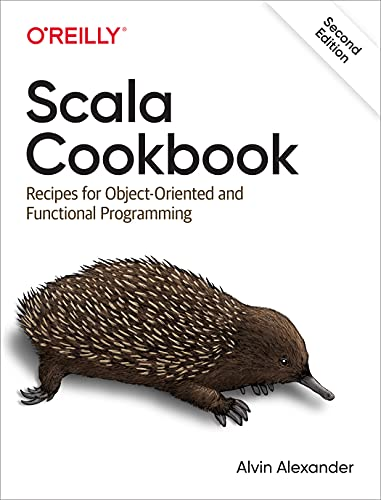
\includegraphics[width=7cm]{paradigm}
            \caption{Scala Cookbook: Recipes for Object-Oriented and Functional Programming} \label{ling2}
            {\tiny \sf Fonte: Amazon Serviços de Varejo do Brasil Ltda.  }
        \end{center}
    \end{figure}
\end{quote}











\chapterimage{Bibliografia.png}
\bibliographystyle{alpha}
\bibliography{scala2}
\addcontentsline{toc}{chapter}{\textcolor{ocre}{Bibliografia}}
%----------------------------------------------------------------------------------------
%	INDEX
%----------------------------------------------------------------------------------------

\cleardoublepage
\phantomsection
\setlength{\columnsep}{0.75cm}
\addcontentsline{toc}{chapter}{\textcolor{ocre}{Index}}
\printindex

%----------------------------------------------------------------------------------------
% Prof. Dr. Ausberto S. Castro Vera
% UENF - CCT - LCMAT - Curso de Ci\^{e}ncia da Computa\c{c}\~{a}o
% Campos, RJ,  2021
% Disciplina: Paradigmas de Linguagens de Programa\c{c}\~{a}o
% Aluno:




\noindent
\textbf{Disciplina:} \textit{Paradigmas de Linguagens de Programa\c{c}\~{a}o \the\year}\\
\textbf{Linguagem:} \textit{Linguagem Scala}\\
\textbf{Aluno:} \textit{Daniel Terra Gomes}


\section*{Ficha de avalia\c{c}\~{a}o:}



\begin{tabular}{|p{12cm}|c|}
  \hline
  % after \\: \hline or \cline{col1-col2} \cline{col3-col4} ...
  \textbf{Aspectos de avalia\c{c}\~{a}o (requisitos m\'{\i}nimos)} & \textbf{Pontos} \\
  \hline
  Elementos b\'{a}sicos da linguagem (M\'{a}ximo: 01 pontos) &  \\
  $\bullet$ Sintaxe (vari\'{a}veis, constantes, comandos, opera\c{c}\~{o}es, etc.) &  \\
  $\bullet$ Usos e \'{a}reas de Aplica\c{c}\~{a}o da Linguagem &  \\
  \hline
  Cada elemento da linguagem (defini\c{c}\~{a}o) com exemplos (M\'{a}ximo: 02 pontos) &  \\
  $\bullet$ Exemplos com fonte diferenciada ( Courier , 10 pts, azul) & \\
  \hline
  M\'{\i}nimo 5 exemplos completos - Aplica\c{c}\~{o}es (M\'{a}ximo : 2 pontos) &  \\
  $\bullet$ Uso de rotinas-fun\c{c}\~{o}es-procedimentos, E/S formatadas &  \\
  $\bullet$ Menu de opera\c{c}\~{o}es, programas gr\'{a}ficos, matrizes, aplica\c{c}\~{o}es &  \\
  \hline
  Ferramentas (compiladores, interpretadores, etc.) (M\'{a}ximo : 2 pontos) &  \\
  $\bullet$ Ferramentas utilizadas nos exemplos: pelo menos DUAS&  \\
  $\bullet$ Descri\c{c}\~{a}o de Ferramentas existentes:  m\'{a}ximo 5&  \\
  $\bullet$ Mostrar as telas dos exemplos junto ao compilador-interpretador&  \\
  $\bullet$  Mostrar as telas dos resultados obtidos nas ferramentas &  \\
  $\bullet$ Descri\c{c}\~{a}o das ferramentas (autor, vers\~{a}o, homepage, tipo, etc.) &  \\
  \hline
  Organiza\c{c}\~{a}o do trabalho (M\'{a}ximo: 01 ponto) &  \\
  $\bullet$ Conte\'{u}do, Historia, Se\c{c}\~{o}es, gr\'{a}ficos, exemplos, conclus\~{o}es, bibliografia &  \\
  \hline
   Uso de Bibliografia (M\'{a}ximo: 01 ponto)&  \\
   $\bullet$ Livros: pelo menos 3&  \\
   $\bullet$ Artigos cient\'{\i}ficos: pelo menos 3 (IEEE Xplore, ACM Library)&  \\
   $\bullet$ Todas as Refer\^{e}ncias dentro do texto, tipo [ABC 04] & \\
   $\bullet$ Evite Refer\^{e}ncias da Internet & \\
   \hline
     &  \\
  Conceito do Professor (Opcional: 01 ponto) & \\
  \hline
   & \\
  \hfill Nota Final do trabalho: & \\
  \hline
\end{tabular}\\
\textit{Observa\c{c}\~{a}o:} Requisitos m\'{\i}nimos significa a \textit{metade} dos pontos


\end{document}
